For the scaling functions we find at this order:
\begin{align}
d_{\tVA,g_4,\Pq}^{(1)} &= d_{\tVA,g_L,\Pq}^{(1)} = 0 = d_{\tAA,2xg_1,\Pq}^{(1)}
\end{align}
and
\begin{align}
d_{\tVV,F_2,\Pq}^{(1)} &= d_{\tAA,F_2,\Pq}^{(1)} 
&d_{\tVV,F_L,\Pq}^{(1)} &= d_{\tAA,F_L,\Pq}^{(1)} 
&d_{\tVA,xF_3,\Pq}^{(1)} &= d_{\tVV,2xg_1,\Pq}^{(1)} 
\end{align}

For $\chi'\to 0$ we find:
\begin{align}
d_{\tVV,F_2,\Pq}^{(1)} &= -\frac{\rho}{9\pi}\left(\DiLog(-\chi) - \frac 1 4 \ln^2(\chi) + \frac{\pi^2}{12} + \ln(\chi)\ln(1+\chi)\right) \nonumber\\
 &\hspace{40pt} + \beta\frac{\rho(718+5\rho)}{2592\pi} + \frac{\rho(232+9\rho^2)}{1728\pi}\ln(\chi) + \mathcal O(\chi')\\
d_{\tVV,F_L,\Pq}^{(1)} &= \left(\beta\frac{-38+23\rho}{54\pi} + \frac{-8+3\rho^2}{36\pi}\ln(\chi)\right)\chi' + \mathcal O({\chi'}^2) \\
d_{\tVV,2xg_1,\Pq}^{(1)} &= d_{\tAA,F_2,\Pq}^{(1)} = d_{\tVA,xF_3,\Pq}^{(1)}\\
d_{\tAA,F_L,\Pq}^{(1)} &= d_{\tVV,F_L,\Pq}^{(1)}
\end{align}

\begin{figure}[ht!]
\centering
\begin{subfigure}[t]{.3\textwidth}
	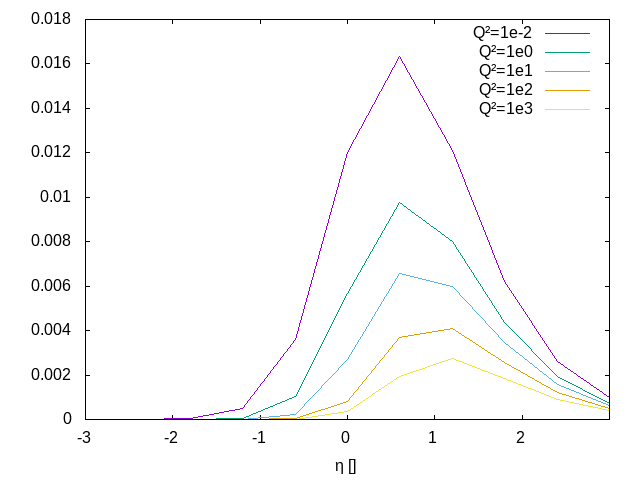
\includegraphics[width=\textwidth]{../../img2/partonic/dq1_VV_F2}
\end{subfigure}%
\begin{subfigure}[t]{.3\textwidth}
	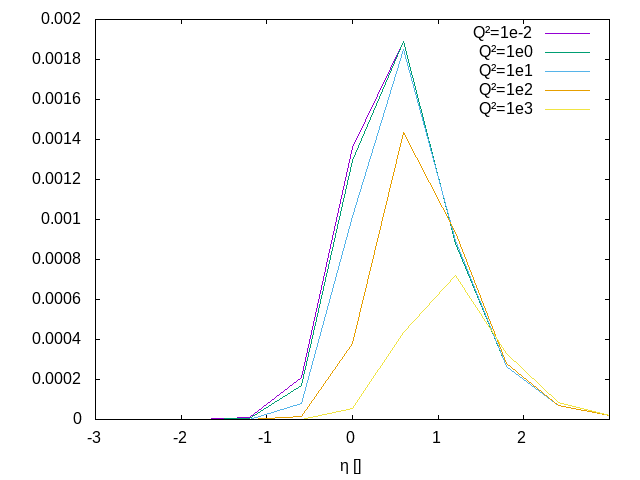
\includegraphics[width=\textwidth]{../../img2/partonic/dq1_VV_FL}
\end{subfigure}%
\begin{subfigure}[t]{.3\textwidth}
	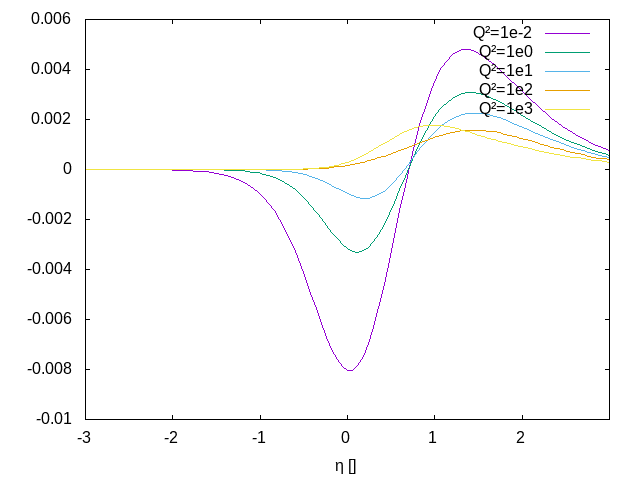
\includegraphics[width=\textwidth]{../../img2/partonic/dq1_VV_x2g1}
\end{subfigure}%
\caption{next-to-leading order scaling functions $\bar c_{k,\Pq}^{(1),F}(\eta,\xi)$ plotted as function of $\eta=s/(4m^2)-1$ for different values of $Q^2$ in units of $\si{\GeV^2}$ at $m=\SI{4.75}{\GeV}$ (i.e. different values of $\xi=Q^2/m^2$) }\label{fig:dq1}
\end{figure}
